\section{Coding}\label{sec:coding}

The central part of the novel genetic approach proposed in this thesis is how an individual is represented.
This is important not only for the construction of the genetic operators, e.g., crossover and mutation
but also for the process of decoding an individual from its representation to the solution.

An individual is represented as a 3D chromosome—which means having three genes—that is composed of
(1) painting sequence random key, (2) slicing order random key, and (3) orientation probabilities.
An example of a chromosome is in figure~\ref{fig:chromosome}.

Let us use the notation for painting sequence random key as $PS_{rk}$,
slicing order random key as $SO_{rk}$,
orientation probabilities as $OR_{prob}$ and instance size as $N$, i.e., number of paintings.
First two are vectors, where $PS_{rk} \in \real^N$ and $SO_{rk} \in \real^{N-1}$.
Orientation probabilities is a matrix where $OR_{prob} \in \real^{N-1, 3}$.
Constraints in~\ref{eq:constraints} apply to each of these parts with
a stochastic vector meaning a vector that contains non-negative elements that add up to one.

\begin{equation}
    \begin{aligned}
        & 1. \quad PS_{rk} \text{ is a stochastic vector.} \\
        & 2. \quad SO_{rk} \text{ is a stochastic vector.} \\
        & 3. \quad \text{Each row in } OR_{prob} \text{ is a stochastic vector.}
    \end{aligned}\label{eq:constraints}
\end{equation}


The above-mentioned representation is based on a solution to the FLP
from~\cite{friedrichIntegratedSlicingTree2018, riponAdaptiveVariableNeighborhood2013},
where the authors represent an individual as a 3D chromosome with concrete identifiers for facilities, slicing order, and orientations.
However, the novel approach to coding proposed in this thesis are (1) the use of the stochastic vectors, (2) the use of random keys, (4) novel mutation and crossover operator, and
(3) introduction of novel decoding of an individual.
Thus, the search in the proposed genetic approach takes place in a different space, which is a space of stochastic vectors.

\begin{figure}[htp]
    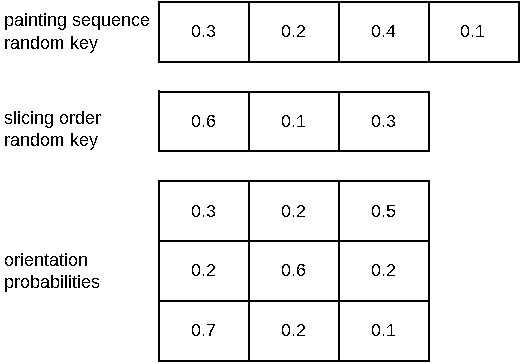
\includegraphics[width=0.8\textwidth, center]{chromosome}
    \caption[Example of an individual representation]{
        Example of an individual representation – two vectors and one matrix.
        Each vector and matrix row form a stochastic vector (vector that contains non-negative elements that add up to one).
    }
    \label{fig:chromosome}
\end{figure}

There are multiple ideas behind representing an individual as a set of stochastic vectors that stem
from extending RKGA~\cite{beanGeneticAlgorithmsRandom1994}, where chromosome is represented as a vector of values from $\langle0,1\rangle$.
First of them is the ability to perform mutation at an arbitrary element of these vectors using
a simple replacement, i.e., substituting an element for a random one from interval $\langle0,1 \rangle$,
followed by normalization back to the stochastic vector.
For example, using representation described in~\cite{friedrichIntegratedSlicingTree2018, riponAdaptiveVariableNeighborhood2013},
there has to be a different mutation method for each part of a chromosome.
By using the representation proposed in this thesis, there has to be only one mutation operator that can be used universally for all parts of the chromosome.

Additionally, when using representations similar to~\cite{friedrichIntegratedSlicingTree2018, riponAdaptiveVariableNeighborhood2013},
after the application of the genetic operators, usually crossover and mutation, an invalid individual might be created.
That is an individual that does not represent any solution.
The presence of invalid individuals might lead to performance loss in FLP~\cite{liuMultiimprovedGeneticAlgorithm2012}.
Moreover, unique solutions for dealing with invalid individuals must be introduced.
For example, left-to-right scan used by~\cite{hwangGeneticAlgorithmApproach2009, kandasamyEffectiveLocationMicro2020}
or leaving invalid individuals inside the population but penalizing them~\cite{hwangGeneticAlgorithmApproach2009}.
The solution proposed in this thesis produces only valid individuals.

Finally, the reasoning behind using a stochastic vector as opposed to a vector from $\langle0,1\rangle$ in RKGA~\cite{beanGeneticAlgorithmsRandom1994}
is the unique implementation of crossover used in this thesis, which is described in subsection~\ref{subsec:crossover}.
